% vim: set filetype=tex spell :

\chapter{Software}
\label{ch:Software}

\section{Overview}

\begin{comment}
\begin{figure}[H]
    \centering
    \begin{tikzpicture}[node distance = 3cm, auto]
        % Place nodes
        \node [block] (AB) {\acs{ARC}bus interface};
        \node [block,right of=AB] (KF) {Kalman Filter};
        \node [block,above of=KF] (alg) {\acs{ACDS} algorithm};
        \node [block,above of=AB] (CMD) {\acs{ACDS} command parse};
        \node [block,right of=alg] (TQ) {Torquer Control and state tracking};
        \node [block,right of=KF] (HC) {House Keeping};
        \node [point,below of=KF] (DN)  {};

        \path [flow] (KF) -- (alg);
        \path [flow] (AB) -- (CMD);
        \path [flow] (alg) -- (TQ);
        \path [flow] (AB) -- (KF);

        %command flow
        \path [flow] (CMD) -- (KF);
        \path [flow] (CMD) -- (alg);

        %house keeping
        \path [flow] (alg) -- (HC);
        \path [flow] (KF) -- (HC);
        \path [flow] (TQ) -- (HC);
        \path [flow] (HC) |- (DN);
        \path [flow] (DN) -| (AB);

    \end{tikzpicture}
    \caption{\acs{ACDS} software overview}
\end{figure}
\end{comment}

\begin{figure}[H]
    \centering
    \begin{tikzpicture}[node distance = 3cm, auto]
        % Place nodes
        \node [block,minimum height=8cm]            (AB) {\acs{ARC}bus interface};

        \node [block,left of=AB,node distance=6cm]  (LEDL) {\acs{LEDL}};
        \node [block,left of=AB,yshift=-3cm]        (CDH) {\acs{CDH}};
        \node [block,left of=CDH]                   (COM) {COM};

        \node [bigblock,right of=AB,node distance=7cm,minimum height=5cm,yshift=1.5cm] (core) {\acs{ACDS} software};
        \node [bigblock,below of=core,node distance=4.5cm,minimum height=2cm] (HC) {House Keeping};


        \path [flow] (AB.58) -- node  {Sensor Data} (core.170);
        \path [flow] (core.190) -- node {Sensor Commands} (AB.48);

        \path [flow] (AB.00) -- node {Ground Station} node [below]{Commands} (core.226);
        \path [flow] (AB.68) -- node {Orbital Elements} (core.140);

        \path [flow] (HC) -- (AB.290);

        \path [flow] (COM) -- (CDH);

        \path [flow] (CDH) -- (AB.250);

        \path [flow] (LEDL.10) -- node  {Sensor Data} (AB.170);
        \path [flow] (AB.190) -- node  {Sensor Commands} (LEDL.350);


    \end{tikzpicture}
    \caption{\acs{ACDS} software overview}
\end{figure}



\section{System Operations Overview}

\autoref{fig:sysopflow} shows the system operations flow. The code starts running after the separation switch is switched and the power system applies power to all systems. Before starting any operations the \ac{ACDS} waits for the on command from the \ac{CDH} board. After the \ac{ACDS} board receives the on command the \ac{ACDS} sends a command to the \ac{LEDL} board to tell it to start taking sensor data. Once sensor data is received the \ac{ACDS} starts to run the detumble algorithm. The Kalman filter needs to know the location of the satellite for it to operate properly so orbital elements must be uploaded before the Kalman filter can start running. Once the Kalman filter knows the location of the satellite it still needs some time to converge to a solution. During this time the \ac{ACDS} remains in detumble mode even if the rates have slowed enoughs to exit. Once the Kalman filter is locked and the rates have sufficiently slowed the \ac{ACDS} switches into mode 2. Mode two is run for a set number \todo{figure out how many and put the number here} of orbits (measured by timing). After mode 2 is complete Mode 3 starts. The \ac{ACDS} remains in mode 3 indefinably unless one of undesirable conditions is detected, see \cite{Mentch11} for details, which causes the \ac{ACDS} to attempt to kick the satellite out of the undesirable alignment and then re-stabilize by transitioning back to mode 2.

\begin{figure}[H]
    \centering
    \begin{tikzpicture}[node distance = 3cm, auto]
    % Place nodes
    \node [block] (sep) {Separation};
    \node [block,below of=sep] (cmd) {On Command from \acs{CDH}};
    \node [block,below of=cmd] (sens) {Send Start Data Collection Command to \acs{LEDL}};
    \node [point,right of=sens,node distance= 3cm]      (p3) {};
    \node [point,right of=sep,node distance= 6cm]       (p4) {};
    \node [block,below of=p4,node distance= 1cm] (detumble) {Detumble};
    \node [point,right of=detumble,node distance= 4cm] (p1) {};
    \node [decision,below of=detumble,node distance = 4cm] (dchk) {Rates and Kalman filter are ready};
    \node [block,below of=dchk,node distance=4cm] (m2) {Mode 2};
    \node [decision,below of=m2,node distance= 3.5cm] (m2chk) {Has Mode 2 time elapsed?};
    \node [point,right of=m2,node distance= 4cm] (p2) {};
    \node [block,below of=m2chk,node distance= 3.5cm] (m3) {Mode 3};
    \node [decision,below of=m3] (cchk) {Correct Alignment?};
    \node [block,right of=cchk,node distance=4cm]  (cor) {apply correction};
    \node [block,above of=cor]  (timer) {reset Mode 2 timer};

    \path[conn] (sep) -- (cmd);
    \path[conn] (cmd) -- (sens);
    \path[line] (sens) -- (p3);
    \path[line] (p3) |- (p4);
    \path[conn] (p4) -- (detumble);

    \path[conn] (detumble) -- (dchk);
    \path[conn] (dchk) --  node [near start] {yes} (m2);
    \path[line] (dchk) -|  node [near start] {no} (p1);
    \path[conn] (p1) -- (detumble);
    \path[conn] (m2) -- (m2chk);
    \path[conn] (m2chk) -- node [near start] {yes} (m3);
    \path[line] (m2chk) -| node [near start] {no} (p2);
    \path[conn] (p2) -- (m2);

    \path[conn] (m3) -- (cchk);
    \path[conn] (cchk) -- node [near start] {no} (cor);
    \path[conn] (cor) -- (timer);
    \path[conn] (timer) |- (m2);

    \path[conn] (cchk.west) -- node [near start] {yes} ([xshift=-1.5cm]cchk.west) |- (m3);

    \end{tikzpicture}
    \caption{System operations chart}
    \label{fig:sysopflow}
\end{figure}

\subsection{Deviations From the flow}

The flow case the flow from \autoref{fig:sysopflow} can be disrupted. This can happen due to commands from the ground station or if the gyros detect that the sattelite is rotating too fast. The ground station can force the \ac{ACDS} into any mode and ether let it go with the normal flow or stay in a particular mode. This allows for recovery in case the system does not function as expected.

If the gyros detect that the satellite is rotating too fast then they will automatically send the \ac{ACDS} into a safe mode where the \ac{ACDS} does not run. It is possible that the \ac{ACDS} could get into a situation where the algorithm speeds up the rotation instead of slowing it down. In this situation the best thing to do is for the \ac{ACDS} to stop and wait for further intervention from the ground.

\section{Incoming Commands\textbackslash Info}

\begin{itemize}
    \item Ground Station Commands
        \begin{itemize}
            \item Uplink Orbit Data
            \item Stop \ac{ACDS}
            \item Force Mode
        \end{itemize}
    \item Sensor Data
\end{itemize}

\section{Software Functions}

\subsection{Torquer Flipping Logic}

\subsection{Data Logging}

During \ac{ACDS} operations data is collected during flight. This data is stored in nonvolatile memory and can be recalled and transmitted to the ground in order to evaluate the \ac{ACDS} system performance. The data that is recorded is shown in \autoref{tab:logdat}

\begin{comment}
\begin{itemize}
    \item magnetometer and gyro readings
    \item torquer status
    \item mode
    \item algorithm intermediate results
    \item torquers flipped
    \item torquer feedback
    \item Kalman filter status
    \item Kalman filter internal variables
    \item Kalman filter state
    \item \todo[inline]{More?}
\end{itemize}
\end{comment}

\begin{table}[H]
    \begin{tabular}{|l|c|c|}
        \hline
        Data&size (bits)&Format\\
        \hline
        mode&2&unsigned integer\\
        \hline
        Time Stamp&32&unsigned integer\\
        \hline
        torquer status&48&flags\\
        \hline
        magnetometer readings&48&unsigned integer (one per axis)\\
        \hline
        gyro readings&36&unsigned integers (one per axis)\\
        \hline
        algorithm intermediate results&TBD&\\
        \hline
        torquers flipped&48&unsigned integer (one per axis)\\
        \hline
        torquer feedback&12&flags\\
        \hline
        Kalman filter status&TBD&\\
        \hline
        Kalman filter internal variables&TBD&\\
        \hline
    \end{tabular}
    \todo[inline]{Resolve DBD's}
    \caption{\ac{ACDS} operations data format}
    \label{tab:logdat}
\end{table}

\subsection{On Board data processing}

Because the downlink data speed is limited, it is necessary to reduce the data that needs to be downlinked. One way to do this is to do some level of on board processing to reduce the data before it is downlinked. For the \ac{ACDS} system this will most likely take the form of returning only the desired data from the recorded data set or returning min/max values from within a data set. 

\subsection{Beacon Data}

The beacon data is transmitted at a fixed rate and provides information about the present state of the satellite. The beacon data could be the only data that is available to diagnose the system. The beacon data must contain enough data to be useful but not so much data that the beacon packets are too big. The beacon data should include raw sensor information as well as information on torquer status. The beacon data from the \ac{ACDS} is shown in \autoref{tab:beacondat}

\begin{comment}
\begin{itemize}
    \item current magnetometer and gyro readings
    \item current torquer status
    \item number of torquer flips so far \todo[inline]{in each axis?}
    \item flags for errors
    \item mode
    \item Kalman filter status
    \item Kalman filter attitude
    \item \todo[inline]{More?}
\end{itemize}
\end{comment}

\begin{table}[H]
    \begin{tabular}{|l|c|c|}
        \hline
        Data&size (bits)&Format\\
        \hline
        current gyro readings&24&signed integers (one per axis)\\
        \hline
        current magnetometer readings&48&signed integers (one per axis)\\
        \hline
        current torquer status&24&flags\\
        \hline
        number of torquer flips so far &&\\
        \hline
        flags for errors&TBD&\\
        \hline
        mode&2&unsigned integer\\
        \hline
        Kalman filter status&TBD&states\\
        \hline
        Kalman filter attitude&64&quaternion\\
        \hline
        Kalman filter rates&48&vector\\
        \hline
    \end{tabular}
    \todo[inline]{Resolve DBD's}
    \caption{Beacon Data format}
    \label{tab:beacondat}
\end{table}

\section{Algorithm Software}

\autoref{fig:swblock} shows the overall software block diagram for the \ac{ACDS} system. Field measurements from the magnetometer are calibrated using the current torquer state and a table of field measurements at different torquer states. The calibrated readings are used to calculate rotation rate and latitude which a long with the field readings are used to calculate the torque that should be applied to the satellite. The torque is then quantized based on \autoref{fig:lpmtq}. The torquers to flip are chosen based current knowledge of torquer stated as well as the desired torque.

\begin{figure}[H]
    \centering
    \begin{tikzpicture}[node distance = 2.6cm, auto]
    % Place nodes
    \node [block] (field) {Magnetic Field Measurements};
    \node [block,right of=field] (cal) {Torquer offset correction};
    \node [point,right of=cal] (split) {};
    \node [block, right of=split,node distance=1.5cm] (alg) {Torque algorithm};
    \node [block, right of=alg] (q) {Torque Quantization};
    \node [block, above of=alg] (rates) {Kalman Filter};
    \node [block,left of=rates,node distance= 3cm] (igrf) {Magnetic field model};
    \node [block,left of=igrf] (pos) {Orbit timing};
    \node [block, below of=alg] (win) {Bias Window Determination};
    \node [point, below of=win] (push) {};
    \node [block, right of=q] (choose) {Choose Torquers to fire};
    \node [point, right of=choose] (fb) {};
    \node [block, right of=fb,node distance=1.5cm] (fire) {Fire Torquers};
    \node [block, below of=choose] (mem) {Torquer Status Tracking};
    \node [block, below of=fire] (sens) {Torquer feedback};

    %draw lines
    \path [conn] (field) -- (cal);
    \path [conn] (split) |- (rates.190);
    \path [conn] (split) |- (win);
    \path [conn] (cal) -- (alg);
    \path [conn] (rates) -- (alg);
    \path [conn] (win) -- (alg);
    \path [conn] (alg) -- (q);
    \path [conn] (q) -- (choose);
    \path [conn] (choose) -- (fire);

    \path [conn] (fb) |- (mem.10);
    \path [phconn] (fire) -- (sens);

    \path [conn] (sens.190) -- (mem.350);
    \path [conn] (mem) -- (choose);
    \path [line] (mem) |- (push);
    \path [conn] (push) -| (cal);

    \path [conn] (pos) -- (igrf);
    \path [conn] (igrf.10) -- (rates.170);


    \end{tikzpicture}
    \caption{Overall Software Block Diagram}
    \label{fig:swblock}
\end{figure}

\subsection{Mode 1}

\begin{comment}
\autoref{fig:mode1} shows the Mode 1 torque algorithm block diagram. In Mode 1 the required torque is simply calculated using rotation rates and field measurements with \autoref{eqn:crossl}. This is also sometimes referred to as the detumble phase because the tumbling motion of the satellite is slowed down to a rate that makes it easier to get into the proper alignment.

\begin{figure}[H]
    \centering
    \begin{tikzpicture}[node distance = 3cm, auto]
    % Place nodes
    \node [input] (field) {Magnetic Field};
    \node [block, right of=field] (alg) { $k {{\vect{\omega}_{err} \cross \vect{B}} \over{\vect{B} \cdot \vect{B}}}$ };
    \node [input, right of=alg] (rates) {Rotation Rates};
    \node [point, below of=alg] (out) {};

    %draw lines
    \path [conn] (field) -- (alg);
    \path [conn] (rates) -- (alg);
    \path [conn] (alg) -- (out);


    \end{tikzpicture}
    \caption{Mode 1 Torque Algorithm Block Diagram}
    \label{fig:mode1}
\end{figure}
\end{comment}

\autoref{fig:mode1} shows the Mode 1 torque algorithm block diagram. In Mode 1 the required torque is calculated using the derivative of the magnetic field. This is a method that is widely used on other CubeSats \todo{Find some B-dot reference(s)} that have magnetic \ac{ACDS}. In this mode the magnetic dipole moment is simply set to a value that is proportional to the derivative of the magnetic field. Because the knowledge of the rotation rates is not needed for Mode 1, detumble can start before the Kalman filter has locked.

\begin{figure}[H]
    \centering
    \begin{tikzpicture}[node distance = 3cm, auto]
    % Place nodes
    \node [input] (field) {Magnetic Field};
    \node [block, right of=field] (alg) { $C {\dot{\vect{B}}}$ };
    \node [point, right of=alg] (out) {};

    %draw lines
    \path [conn] (field) -- (alg);
    \path [conn] (alg) -- (out);


    \end{tikzpicture}
    \caption{Mode 1 Torque Algorithm Block Diagram}
    \label{fig:mode1}
\end{figure}
\subsection{Mode 2}

\autoref{fig:mode2} shows the Mode 2 torque algorithm block diagram. Torque is calculated the same way as in Mode 1 but this time a bias is added depending on which region of the orbit the satellite is in. The bias tends to cause the satellite to rotate. This causes the algorithm to cancel out the bias. This is prevented by preventing the resulting dipole moment from being in the opposite direction as the bias. Outside of the bias regions the torquers are set to produce no torque.

\begin{figure}[H]
    \centering
    \begin{tikzpicture}[node distance = 3cm, auto]
    % Place nodes
    \node [input] (field) {Magnetic Field};
    \node [block, right of=field] (alg) { $k {{\vect{\omega}_{err} \cross \vect{B}} \over{\vect{B} \cdot \vect{B}}}$ };
    \node [input, right of=alg] (rates) {Rotation Rates};
    \node [oppr,below of=alg,node distance=2cm] (sum) {+};
    \node [block,left of=sum,node distance=3cm] (bias) {Mode 2 bias table};
    \node [input,left of=bias] (win) {Bias Window};
    \node [block,below of=sum,node distance=2cm] (fix) {Bias Fix};
    \node [block,below of=fix,node distance=2.5cm] (coast) {Coast?};
    \node [point, below of=coast] (out) {};

    %draw lines
    \path [conn] (field) -- (alg);
    \path [conn] (rates) -- (alg);
    \path [conn] (alg) -- (sum);
    \path [conn] (win) -- (bias);
    \path [conn] (bias) -- (sum);
    \path [conn] (sum) -- (fix);
    \path [conn] (fix) -- (coast);
    \path [conn] (win) |- (coast);
    \path [conn] (coast) -- (out);

    \end{tikzpicture}
    \caption{Mode 2 Torque Algorithm Block Diagram}
    \label{fig:mode2}
\end{figure}

\subsection{Mode 3}

\autoref{fig:mode3} shows the Mode 3 torque algorithm block diagram. This is similar to Mode 2 except only the north pole bias window is used and outside the bias window torque is generated to slow rotation rates.

\begin{figure}[H]
    \centering
    \begin{tikzpicture}[node distance = 3cm, auto]
    % Place nodes
    \node [input] (field) {Magnetic Field};
    \node [block, right of=field] (alg) { $k {{\vect{\omega}_{err} \cross \vect{B}} \over{\vect{B} \cdot \vect{B}}}$ };
    \node [input, right of=alg] (rates) {Rotation Rates};
    \node [oppr,below of=alg,node distance=2cm] (sum) {+};
    \node [block,left of=sum,node distance=3cm] (bias) {Mode 3 bias table};
    \node [input,left of=bias] (win) {Bias Window};
    \node [block,below of=sum,node distance=2cm] (fix) {Bias Fix};
    \node [point, below of=fix] (out) {};

    %draw lines
    \path [conn] (field) -- (alg);
    \path [conn] (rates) -- (alg);
    \path [conn] (alg) -- (sum);
    \path [conn] (win) -- (bias);
    \path [conn] (bias) -- (sum);
    \path [conn] (sum) -- (fix);
    \path [conn] (fix) -- (out);


    \end{tikzpicture}
    \caption{Mode 3 Torque Algorithm Block Diagram}
    \label{fig:mode3}
\end{figure}

\subsection{Mode Switching}

Mode switching on \ac{ARC} will be time based. The original simulation used the rotation rates to switch from Mode 1 mode to Mode 2 but it was found that when the satellite did not have full knowledge of rotation rates, as will be the case if they are determined from magnetic field, then the mode was switched too soon. The switch from Mode 2 to Mode 3 is timed to be about 10 orbits after the switch into Mode 2. Once in Mode 3 no more automated mode switching is done. Modes can also be switched at all times via ground station command.

\begin{comment}
\subsection{Bias Window Determination}

\autoref{fig:biaswin} shows how the bias window determination will work. To determine where \ac{ARC} is within the orbit, peaks are found in the magnitude of the magnetic field. The field magnitude is used because it is independent of attitude. The magnitude of the field is greatest at the south pole but the magnetic north pole is located closer to the geographic north pole so it's peaks are more consistent. South pole peaks are filtered out first by eliminating peaks that are ether too high or too low to be a north pole peak. Peaks are further filtered by tracking the timing of past peaks and rejecting peaks that happen too soon. If a second peak is detected very soon after a north pole peak then it is assumed to be a double peak and the average peak time is taken. After the north poles are found the orbital period can be determined and orbital progress can be tracked. The current bias window is determined using the current orbital progress and a lookup table. In case the automatic orbit tracking does not work properly it is possible to upload timing parameters for the orbit tracking to use instead.

\begin{figure}[H]
    \centering
    \begin{tikzpicture}[node distance = 3cm, auto]
    % Place nodes
    \node [input] (field) {Field Measurements};
    \node [block,below of=field,node distance=2.1cm] (mag) {Vector Magnitude};
    \node [block,right of=mag] (peak) {Peak Detect};
    \node [block,right of=peak] (level) {Level Check};
    \node [block,right of=level] (pole) {North Pole Detect};
    \node [block,right of=pole] (gen) {Orbit tracking};
    \node [block,below of=gen,node distance=2.5cm] (time) {Timing Source};
    \node [block,above of=gen] (upload) {Timing Parameter Upload};
    \node [block,right of=gen] (lookup) {Bias Window Lookup};
    \node [point,right of=lookup,node distance=2cm] (out) {};

    %draw lines
    \path [conn] (field) -- (mag);
    \path [conn] (mag) -- (peak);
    \path [conn] (peak) -- (level);
    \path [conn] (level) -- (pole);
    \path [conn] (pole) -- (gen);
    \path [conn] (gen) -- (lookup);
    \path [conn] (lookup) -- (out);
    \path [conn] (time) -- (gen);
    \path [conn,dashed] (upload) -- (gen);

    \end{tikzpicture}
    \caption{Bias Window Determination Block Diagram}
    \label{fig:biaswin}
\end{figure}

\end{comment}

\begin{comment}
\subsection{Rotation Rate Calculations}

The rotation rate is calculated using the magnetic field measurements. \autoref{eqn:magrate} shows how to calculate the rotation rate using magnetic field measurements. In \autoref{eqn:magrate} $\dot{\vec{B}}$ is calculated using there magnetic field measurements and the central difference formula as suggested in \cite{Mentch11}.

\begin{equation}
    %TODO: add dot over B
    \vec{\omega}={\dot{\vec{B}} \cross \vec{B} \over{\vec{B} \cdot \vec{B}}}
    \label{eqn:magrate}
\end{equation}
\end{comment}

\subsection{Kalman Filter}

\begin{figure}[H]
    \centering
    \begin{tikzpicture}[node distance = 3cm, auto]
    % Place nodes
        \node [block] (pstate) {Project State};
        \node [block,below of=pstate] (pcov) {Project Error Covariance Ahead};
        \node [block,right of=pcov] (gain) {Compute Kalman Gain};
        \node [block,right of=gain] (ustate) {Update state Estimate};
        \node [input,right of=ustate,text width = 3cm,node distance=3.5cm] (meas) {Measurement Input};
        \node [block,above of=ustate] (ucov) {Update Error Covariance};


    %draw lines

    \path [conn] (pstate) -- (pcov);
    \path [conn] (pcov) -- (gain);
    \path [conn] (gain) -- (ustate);
    \path [conn] (meas) -- (ustate);
    \path [conn] (ustate) -- (ucov);
    \path [conn] (ucov) -- (pstate);


    \end{tikzpicture}
    \caption{Extended Kalman Filter}
    \label{fig:eKalman}
\end{figure}

\section{Support Software}

\subsection{Torquer Calibration}

Because the torquers produce a magnetic field and are in close proximity to the magnetometer the effects of the torquers must be calibrated out. This is possible because the magnetic field of the torquers have a small number of discrete states and these states are fairly repeatable \todo{Test repeatability}

Because the torquer offsets depend on the geometry of the torquers and magnetometer(s), the offsets must be calculated after the satellite has been fully integrated. To calculate the offsets the satellite is placed in the Helmholtz cage and connected to the Helmholtz Cage Computer. A Matlab script is run that runs the calibration procedure for each combination of torquer states to calculate the offset at each state. 

\subsubsection{Calibration Testing}

To test how well the calibration functions a testing script was written. \autoref{fig:tcalTst} shows a plot from the test script. To run the test script the fully integrated satellite is placed in the Helmholtz cage. The script sweeps the magnetic field of the Helmholtz cage through a predefined field sequence taking magnetic field readings at each step. At fixed intervals the satellite is told to flip a random torquer in each axis in a random direction. The previously defined correction data for the torquers is used to compute what the external field is. For comparison the readings are also plotted with just the scale factor correction. The difference in readings is very apparent as can be seen in \autoref{fig:tcalTst}.


\begin{figure}[H]
    \centering
    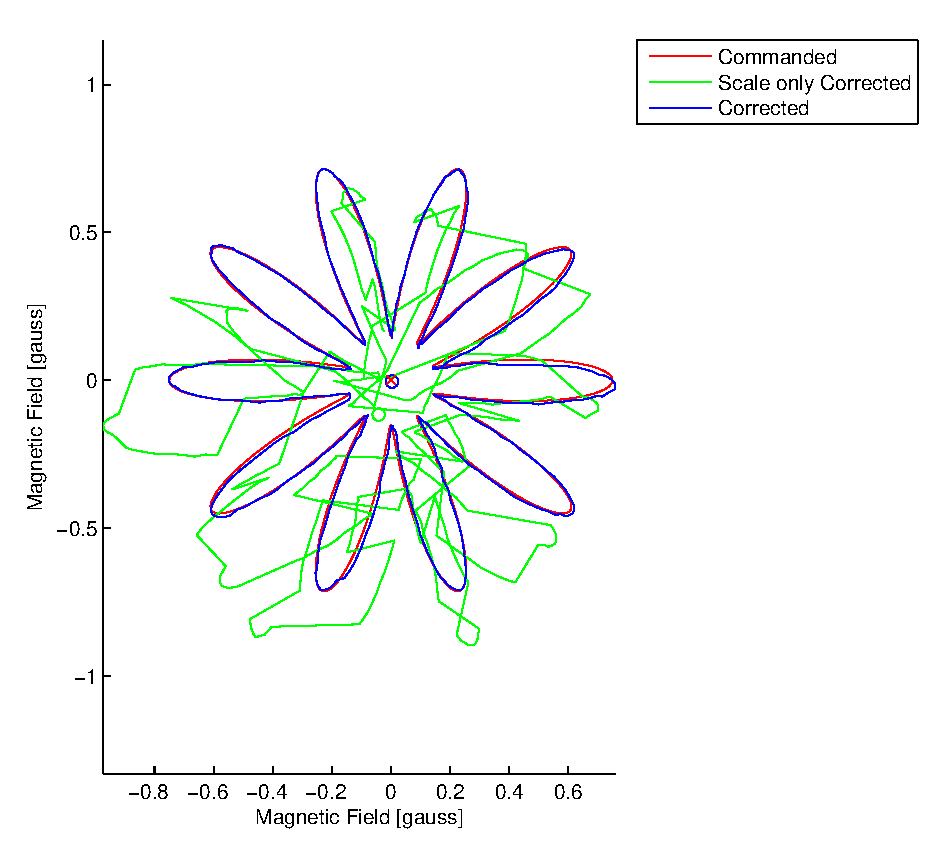
\includegraphics[width=\textwidth]{Figures/torqueCalTst}
    \caption{Torquer Calibration Test Graph}
    \label{fig:tcalTst}
    \todo[inline]{Repeat with fully integrated satellite as it says in the text.}
\end{figure}

\todo[inline]{Try to quantify error introduced by torquers and discuss}

\subsection{Feedback Software}

The feedback comparators are sampled before and after the torquer is flipped to check the capacitor status. If the torquer has been successfully flipped the capacitor will be charged before the flip happened and discharged afterwards, otherwise there was an error. 


